\documentclass[conference]{IEEEtran}
\IEEEoverridecommandlockouts

% ==== Fonts & core packages ====
\usepackage{newtxtext,newtxmath}
\usepackage{graphicx}
\usepackage{amsmath}
\usepackage{cite}
\usepackage{tikz}
\usetikzlibrary{arrows.meta,positioning}
\usepackage{xcolor}
\usepackage[hidelinks]{hyperref}

% TikZ styles for figures
\tikzset{
  metal/.style={draw, fill=gray!18},
  gate/.style={draw, rounded corners=1pt, fill=blue!7},
  chan/.style={draw, thick},
  oxide/.style={draw, dashed, fill=orange!8},
  via/.style={draw, fill=black!25},
  contact/.style={draw, fill=gray!35},
  lab/.style={font=\scriptsize},
  tinycap/.style={font=\scriptsize, align=center}
}

% Safe resize helper
\newcommand{\fitfig}[1]{\resizebox{0.92\linewidth}{!}{#1}}

\title{Educational Perspectives on Complementary FETs (CFET):\\
Evolution Beyond GAA and Open Challenges}

\author{
\IEEEauthorblockN{Shinichi Samizo}
\IEEEauthorblockA{Independent Semiconductor Researcher\\
Project Design Hub, Samizo-AITL\\
\textit{Email:} \href{mailto:shin3t72@gmail.com}{shin3t72@gmail.com}\quad
\textit{GitHub:} \href{https://github.com/Samizo-AITL}{Samizo-AITL}}
}

\begin{document}
\maketitle

\begin{abstract}
This tutorial paper provides an educational overview of emerging
\emph{Complementary FET (CFET)} technology, which vertically stacks nFET and pFET devices beyond Gate-All-Around (GAA) nanosheets.
CFET reframes the CMOS inverter as a \emph{cross-sectional} integration, promising density and delay improvements.
We consolidate structure, electrostatic motivations, layout and delay impacts, fabrication challenges, and modeling limitations, and articulate the pedagogical value of CFET as an open, unresolved technology for semiconductor curricula.
\end{abstract}

\begin{IEEEkeywords}
CFET, GAA, FinFET, nanosheet FET, short-channel effects, scaling, education, tutorial, vertical stacking, PDK.
\end{IEEEkeywords}

% =========================
\section{Introduction}
Scaling has progressed from planar CMOS to FinFET and most recently GAA nanosheet FETs.
Beyond the 2\,nm node, interconnect delay and cell footprint limit further gains despite excellent electrostatics.
CFET stacks nFET and pFET in the vertical dimension so that the cross-section itself constitutes a CMOS inverter, potentially doubling effective standard-cell density while shortening n--p connections.
This paper positions CFET as both a roadmap element and an educational vehicle for device--design co-optimization.

% =========================
\section{Device Evolution: From SCE Relief to Cross-Sectional CMOS}
\subsection{Planar CMOS and SCE Motivation}
As gate lengths entered the deep sub-100\,nm regime, planar MOSFETs suffered
from short-channel effects (SCE): threshold-voltage roll-off, drain-induced barrier lowering, off-state leakage, and degraded subthreshold slope.
Electrostatic control by a single top gate could no longer effectively pinch off the channel.

\subsection{FinFET: Three-Sided Gate Control}
FinFETs improved electrostatics by wrapping the gate around \emph{three} sides of a vertical fin.
The stronger gate-to-channel coupling sharpened subthreshold slope and reduced variability.
Drive current density per footprint increased by using multiple fins per device.
However, the tall/narrow fin introduced process complexity and left one side of the channel uncontrolled.

\subsection{GAA Nanosheet: Four-Sided Control}
Gate-All-Around (GAA) nanosheet FETs extend control to \emph{four} sides by surrounding suspended sheets with the gate.
This architecture strongly suppresses SCE and variability and allows gate-length scaling to continue.
Yet, the design bottleneck shifted from device electrostatics to \emph{interconnect}: RC delay and lateral footprint of standard cells.

\subsection{CFET: Stacking Complementary Devices}
CFET addresses wiring and density limits by placing nFET and pFET in the \emph{same lateral footprint} and connecting them vertically.
Two educational takeaways are:
(i) cell density can approach $\sim 2\times$ by sharing diffusion/gate footprint across polarities; and
(ii) the critical n-to-p inverter connection shortens to a vertical via, reducing RC delay.
CFET reframes CMOS as a \emph{cross-sectional inverter}.

\begin{figure}[htbp]
\centering
\fitfig{%
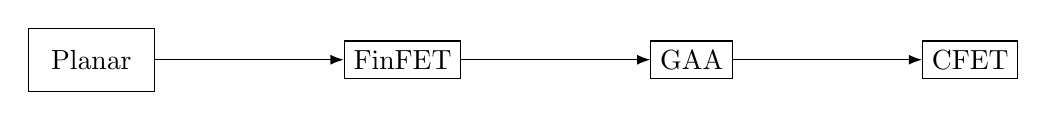
\begin{tikzpicture}[node distance=2.4cm,>=Latex]
\node[draw, minimum width=1.6cm, minimum height=0.8cm] (planar) {Planar};
\node[draw, right=of planar] (finfet) {FinFET};
\node[draw, right=of finfet] (gaa) {GAA};
\node[draw, right=of gaa] (cfet) {CFET};
\draw[->] (planar) -- (finfet);
\draw[->] (finfet) -- (gaa);
\draw[->] (gaa) -- (cfet);
\end{tikzpicture}}
\caption{Device evolution by electrostatics and wiring: Planar $\rightarrow$ FinFET (3-side) $\rightarrow$ GAA (4-side) $\rightarrow$ CFET (vertical stack).}
\label{fig:evolution}
\end{figure}

% =========================
\section{CFET Structural Concepts}
\paragraph*{(i) Sequential CFET}
nFET is fabricated first, followed by pFET under a constrained thermal budget.
Selective epitaxy/etch and tier isolation are crucial, as is vertical contact to the inverter output.

\begin{figure}[htbp]
\centering
\fitfig{%
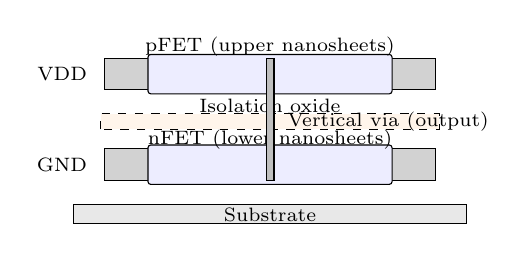
\begin{tikzpicture}[x=1cm,y=1cm]
% Substrate
\draw[metal] (0,0) rectangle (5,0.25);
\node[tinycap] at (2.5,0.12) {Substrate};

% nFET (lower)
\draw[contact] (0.4,0.55) rectangle (1.0,0.95);
\draw[contact] (4.0,0.55) rectangle (4.6,0.95);
\foreach \y in {0.62,0.74,0.86}{
  \draw[chan] (1.0,\y) -- (4.0,\y);
}
\draw[gate] (0.95,0.5) rectangle (4.05,1.0);
\node[lab] at (2.5,1.07) {nFET (lower nanosheets)};

% Isolation oxide
\draw[oxide] (0.35,1.20) rectangle (4.65,1.40);
\node[lab] at (2.5,1.50) {Isolation oxide};

% pFET (upper)
\draw[contact] (0.4,1.70) rectangle (1.0,2.10);
\draw[contact] (4.0,1.70) rectangle (4.6,2.10);
\foreach \y in {1.77,1.89,2.01}{
  \draw[chan] (1.0,\y) -- (4.0,\y);
}
\draw[gate] (0.95,1.65) rectangle (4.05,2.15);
\node[lab] at (2.5,2.25) {pFET (upper nanosheets)};

% Vias
\draw[via] (2.45,0.55) rectangle (2.55,2.10);
\node[lab, anchor=west] at (2.6,1.3) {Vertical via (output)};

% Power rails
\node[lab, anchor=east] at (0.3,0.75) {GND};
\node[lab, anchor=east] at (0.3,1.90) {VDD};
\end{tikzpicture}}
\caption{Sequential CFET cross-section: pFET stacked over nFET with vertical output via and tier isolation.}
\label{fig:cfet_stack}
\end{figure}

\paragraph*{(ii) Forksheet CFET}
n/p channels are placed orthogonally with a dielectric ``fork'' spacer to ease routing congestion and preserve electrostatics.

\begin{figure}[htbp]
\centering
\fitfig{%
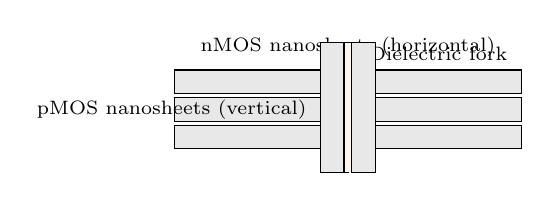
\begin{tikzpicture}[x=1cm,y=1cm]
% nMOS sheets (horizontal)
\foreach \y in {0.2,-0.15,-0.5}{
  \draw[metal] (-2.2,\y) rectangle (2.2,\y+0.3);
}
\node[lab,anchor=south] at (0,0.55) {nMOS nanosheets (horizontal)};

% fork spacer
\draw[oxide] (-0.10,-0.80) rectangle (0.10,0.85);
\node[lab,anchor=west] at (0.15,0.70) {Dielectric fork};

% pMOS sheets (vertical)
\draw[metal] (-0.35,-0.80) rectangle (-0.05,0.85);
\draw[metal] (0.05,-0.80) rectangle (0.35,0.85);
\node[lab,anchor=east] at (-0.40,0.00) {pMOS nanosheets (vertical)};
\end{tikzpicture}}
\caption{Forksheet-CFET top view: orthogonal n/p nanosheets separated by dielectric fork for routing relief.}
\label{fig:forksheet}
\end{figure}

% =========================
\section{Electrical and Layout Impacts}
Key educational points:
\begin{itemize}
  \item \textbf{Area efficiency:} Near $\sim 2\times$ density for inverter cells; benefits extend to NAND/NOR by co-locating pull-up and pull-down networks.
  \item \textbf{Delay/energy:} Vertical n-to-p via shortens RC path; FO1 delay improves even if single-device $I$-$V$ matches GAA.
  \item \textbf{Electrostatics:} Tiers retain GAA control; inter-layer coupling adds parasitics.
  \item \textbf{Variability/noise:} Thermal coupling and VDD/GND partitioning introduce asymmetries requiring placement and routing co-optimization.
\end{itemize}

% =========================
\section{Manufacturing Challenges}
Stacked tiers demand selective epitaxy/etch, low thermal budgets, and precise alignment.
Dielectric isolation must block dopant diffusion while supporting vias.
BEOL co-design ensures VDD/GND distribution and output via landing without track penalties.

% =========================
\section{Modeling and EDA Limitations}
BSIM-CMG captures GAA but not CFET-specific vertical coupling or thermal effects.
Verilog-A prototypes exist without consensus.
No open CFET PDKs or standard-cell libraries are available, leaving CFET as an open sandbox for education.\nocite{*}

% =========================
\section{Educational Value}
CFET connects device physics with circuit/layout co-design.
It exposes students to unresolved challenges in fabrication, modeling, and CAD---a rich basis for advanced device courses, design projects, and capstone activities.

% =========================
\section{Conclusion and Outlook}
CFET reframes CMOS as a stacked, cross-sectional inverter.
Beyond electrostatics, it targets wiring delay and density.
Future vectors include forksheet layouts, 3D-CFET, thermal-aware power partitioning, and System-on-Stack.
Embedding CFET in curricula prepares engineers for the 2030s.

\section*{Acknowledgment}
The author thanks the Project Design Hub community for discussions.

\bibliographystyle{IEEEtran}
\bibliography{refs}

\section*{Author Biography}
\noindent\textbf{Shinichi Samizo}
received the M.S. degree in Electrical and Electronic Engineering from Shinshu University, Japan.
He worked at Seiko Epson Corporation as an engineer in semiconductor memory and mixed-signal device development, and contributed to inkjet MEMS actuators and PrecisionCore printhead technology.
He is currently an independent semiconductor researcher focusing on process/device education, memory architecture, and AI system integration.\\[2pt]
\textbf{Contact:} \href{mailto:shin3t72@gmail.com}{shin3t72@gmail.com}, \href{https://github.com/Samizo-AITL}{Samizo-AITL}

\end{document}
